\secput*{Preprocessing}

This section describes how a range coalescing data structure is built cache-obliviously
from a set of $k$ $n$-length sorted lists $L_1 \ldots L_k$ and bounds
the number of memory transfers incurred by the process.  We do this in four steps.
First, we give a suboptimal deterministic strategy for finding the splitters 
--- the values that partition the query space such that each partition has $O(k)$ 
elements from the constituent lists in $\{ L_1 \ldots L_k \}$.  Second, we 
demonstrate that the elements from each list can be assembled in the bin corresponding
to each splitter using $O(nk / B)$ memory transfers.  Finally, we give two randomized
algorithm for finding the splitters when $k < \lg^2 n$ and $k \geq \lg^ n$, 
respectively, each of which incurs $O(nk/B)$ memory transfers.  

\subsection*{Preprocessing suboptimally}

In this section, we show how to find an $n$-length sorted splitter array $S$, such that $O(k)$
elements from $\mathcal{L} = \cup_{i=1}^{k}L_i$ fall in each range 
$[S_j,S_{j+1})$ $\forall j$.  If we assume that all elements in $\mathcal{L}$ are 
unique, we can merely merge all the elements and take every $k$th element in the
merged list as the splitters.  \footnote{We can extend the value of each element with the
list number in order to make them unique, since the elements from any particular
list $L_i$ are unique.  Note that if each list contained a value $l$ and the
value $l$ from
the $L_i$ was chosen as the $j$th splitter $S_j$, we do not compromise the correctness of the 
query, since the next smaller value than $S_j$ from each list in $\{ L_1 \ldots L_k\}$ is 
contained in the $j$th bin.} We can use a cache-oblivious 
$k$-merger~\cite{FrigoLePr99} to merge the elements using 
$O((nk/B) \log_{M/B} (k/B) + k)$ memory transfers if $k \leq \sqrt[3]{n}$ and
$O((nk/B) \log_{M/B} (nk/B))$ memory transfers otherwise.



\subsection*{Bin construction}

This section demonstrates how we can build the $O(k)$-sized bin corresponding to each splitter
in the array $S$ using $O(nk/B)$ memory transfers in the worst case.
If we were to merely build each of the $n$ bins in sequence, each of which could
incur as many as $2k$ memory transfers since $k$ may be larger than $M$, we could
incur as many as $O(nk)$ memory transfers overall.  This is unacceptable.  
Instead, we will build the bins using a $Z$-order traversal~\cite{Morton66} of 
the 2D space spanned by the cross-product of bin number and list number.

SNARF: optionally include a graphic of z-order, labeled with bin number, list number
and depicting that we have $ac$ blocks in cache to handle a $c$ by $c$ space.

\begin{figure}[h]
%\begin{center}
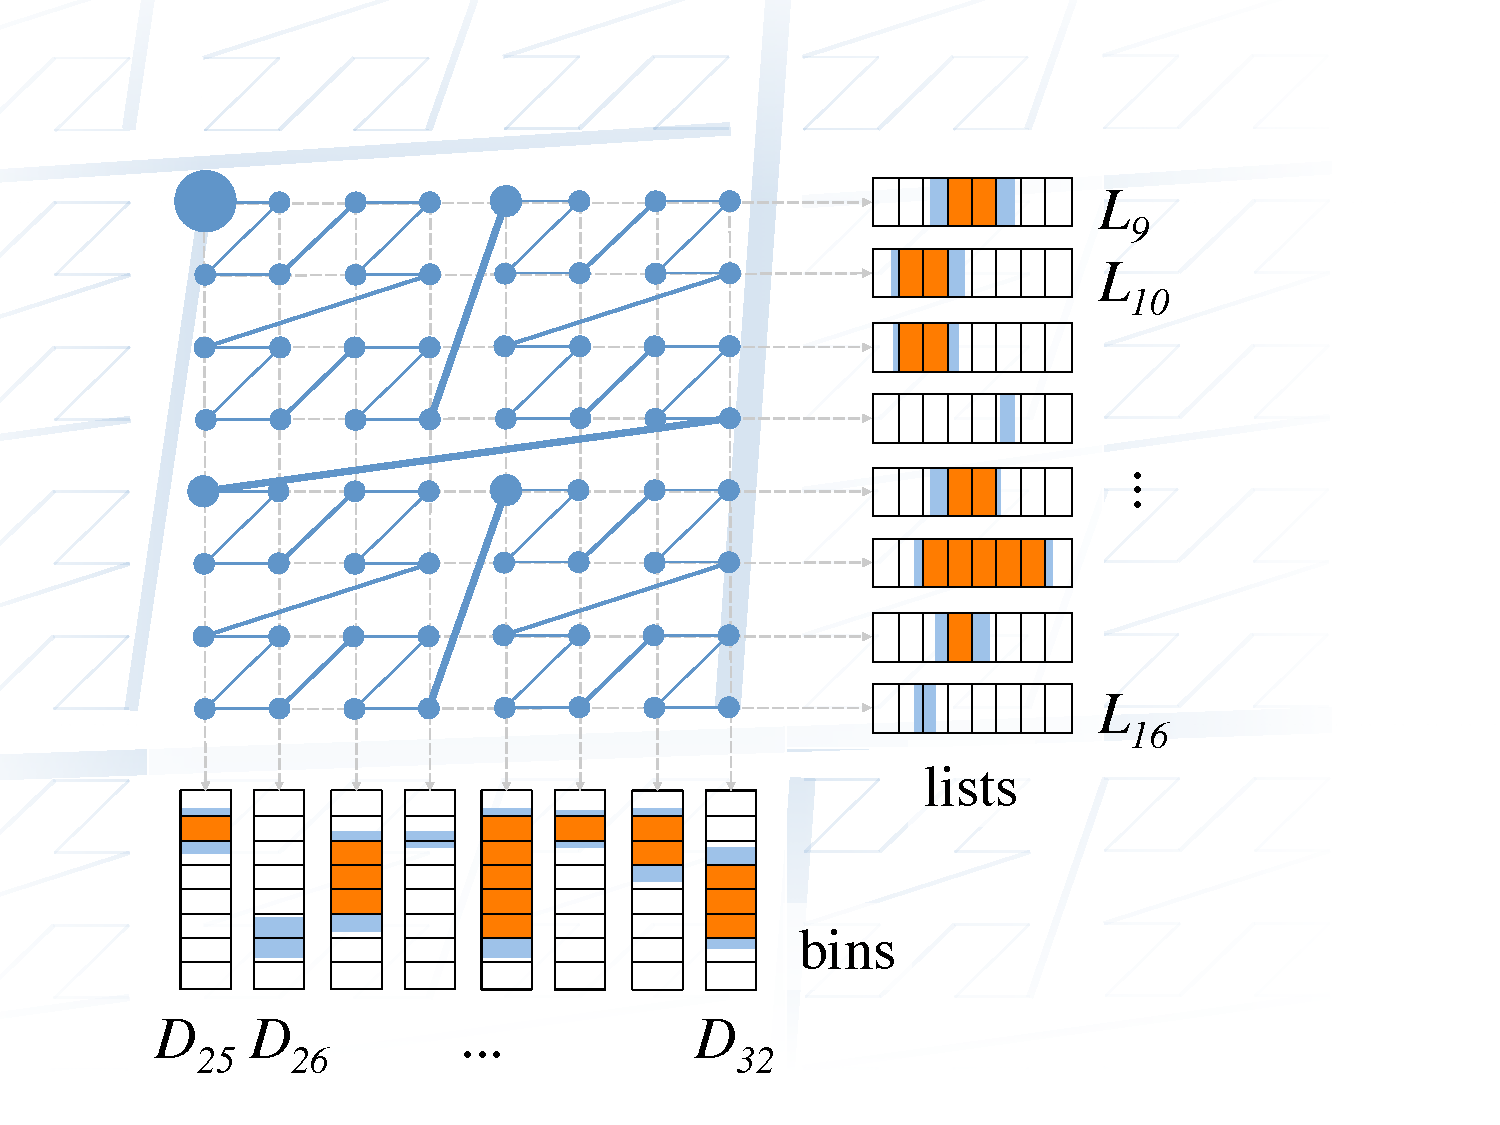
\includegraphics[scale=.35]{bin-construction.pdf}
%\end{center}
\caption{}
\label{fig:range_coalescing} 
\end{figure}


\begin{theorem}
Given a sorted list of $O(n)$ splitters $S$ and $k$ sorted $n$-length lists 
$L_1 \ldots L_k$, the bins for a range coalescing data structure can be constructed
deterministically and cache-obliviously using $O(nk/B)$ memory transfers.
\end{theorem}

\begin{proof}
Consider a $2^r$ by $2^r$ naturally aligned region in the iteration space of the
cross product of bin number and list number\footnote{A naturally aligned region
of size $c$ by $c$ is one which begins with some indices $i \equiv 1 \pmod{c}$ 
in one dimension and $j \equiv 1 \pmod{c}$ in the other.}.  
The cache need only keep the head of each of the $2^r$ constituent
lists $L_{i2^r + 1} \ldots L_{(i+1)2^r}$ for some $i$ and the head of the $2^r$ bins 
$D_{j2^r + 1} \ldots D_{(j+1)2^r}$ for some $j$. 
The ''head'' of a list is the current location
in the list as the list is streamed linearly to transfer the elements to various bins.  
For the head of each list, there can be as many as
two non-full memory tranfers (ie. not all of the elements on the cache block were
written or read).  Consider the largest $r$ for which these $2 \cdot 2^r$ list heads
fit in cache, so that $a2^r = M$ for some constant $a$.  In total, there will be 
$nk/2^{2r}$ cache flushes for a total of $M \cdot nka^2/M^2 = O(nk/B)$ cache blocks, 
assuming $M = \Omega(B)$.  There may also be additional full memory transfers in the
course of processing each $2^r$ by $2^r$ region, though
each element may appear in at most one full memory transfer, thus there are at most
$nk/B$ full memory transfers.  
\end{proof}

\subsection*{Finding splitters for small $k$}

$k < \lg^2 n$

In this section, sample every element with probability $1/k$ and we just subdivide any bins
with more than $2(1+\epsilon)k$ elements with a cache-oblivious select algorithm.
The total number of memory transfers is $O(N/B)$ whp, which we get through a Hoeffding
bound.

Show that the number of splitters is $O(n)$ - Chernoff.

\subsection*{Finding splitters for large $k$}

$k \geq \lg ^2 n$

In this section, we use sample sort (randomly select with probability $1/\lg k$ and
then rake exactly $N/k$ evenly spaced samples) and $k$ is large enough that we don't have
to subdivide the bins, yet still get $O(k)$-sized (actually, at most 
$2(1+\epsilon)k$ elements) bins whp.  



